%%%%%%%%%%%%%%%%%%%%%%%%%%%%%%%%%%%%%%%%%%%%%%%%%
%%%%%%%%%%%% chap: Implementation \& Results%%%%%%%%%%%%%%%%%
%%%%%%%%%%%%%%%%%%%%%%%%%%%%%%%%%%%%%%%%%%%%%%%%%

\chapter{Implementation Logic}\label{chapter:chap4}

\section{System Requirments \& Technologies Used}\label{sect:System Requirments \& Technologies Used}

For the implementation of the proposed app, the development medium chosen was Android Studio, while the programming language used was Kotlin. Details on all technologies used are as follows:\\

\textbf{\ac{IDE} used: }  \\
Android Studio \cite{1} is an official \ac{IDE} for Android app development, based on the tools offered by the IntelliJ IDEA, which is designed with powerful features for increased productivity in app development. The features on offer by Android Studio are as follows: a Gradle-based build system, an emulator for testing and experimenting on the apps developed, offering for the user the ability to test his or her application on different \ac{API} levels, and personalize their emulator settings for varied testing environments, the ability to develop applications for all Android devices, the ability to edit and update composables in real-time while the emulator or physical device is running. The \ac{IDE} also offers different code templates, testing tools, and frameworks for an increase in productivity and development time, while also including a GitHub integration and support for C++ and \ac{NDK}.
\\

\textbf{Programming Language used: } \\
Kotlin \cite{5} is a cross-platform, general-purpose programming language developed and released in 2011 by JetBrains, being built as a statically typed language, meaning that the variable type is going to be known at compile time. One key feature of Kotlin is in its design policy, the language being developed to be fully interoperable with Java, making the use of Java and Kotlin, in the same project, possible. With it being a concise, and safe programming language, it is usually recommended the use of Kotlin in applications development, being more often than not the best choice for such projects. The main reasons why Kotlin is a good choice for development stems from its many features that allow its users to write code in an easier manner, such as null safety, coroutines used for asynchronous programming, and extension functions. 

\newpage

\textbf{Database technology used: } \\

Firebase \cite{2} is an app development platform that offers a variety of tools and services to help in the development of high-quality applications. 

One of the key features of Firebase is the Firebase Realtime Database \cite{3}, which is a cloud-hosted database. The data is stored in a \ac{JSON} file, letting the user store and sync data in real-time, for every connected client. Such features help when building cross-platform applications, with all clients sharing one Realtime Database instance and automatically receiving updates with the newest data.

\textbf{Other technology used: } \\

Other technologies used include the Jetpack Compose toolkit, used for the UI layout, and the use of XML files which were used for certain screen layouts, strings, color pallets, permission, component definition, various graphical elements, and so on.

Jetpack Compose \cite{4} is a toolkit designed for building Android \ac{UI}. Its main benefits consist of simplifying and accelerating \ac{UI} development on Android by allowing by providing the user with a set of powerful tools, and intuitive Kotlin \ac{API}s, being fully declarative, which means that the \ac{UI} elements can just be described and Compose will take care of the rest. Another big benefit of Compose is that the \ac{UI} automatically updates.

XML files are used in Android Studio and app development for several purposes, such as:\\
    • Layout: This type of XML file is used to define the general layout of the user interface, holding all elements such as text views, buttons, sliders, and others;\\
    • Strings: This file is used as an alternative for hard-coded strings. They define strings that can be accessed throughout the entire app, being especially useful for changing the text of an app from one language to another;\\
    • Colors: This XML file is used to define different colors that the user can use throughout the application, this file is especially useful when changing the theme of an app;\\
    • Drawables: These are XML files that are used to create various graphic icons or images;
    • Manifest: Lastly, these files are used to define the components of the application, including the packages, activities, receivers, and permissions that the application needs;\\
\\
For testing, the app was experimented on the emulators provided by Android Studio, on an emulator with \ac{API} 30 and 33, and the app was also tested on different physical devices, mainly a Samsung J6, and a Samsung A 54.

The basic system requirements for running the app are as follows:

    • An Android phone with the Android Version 11+;
    
    • Connection to the Internet;
\newpage
\section{Implementation}\label{sect:Implementation}

\subsection{Main Menu Implementation}\label{subsect:Main Menu Implementation}

\begin{figure}[htp]
    \centering
    \begin{minipage}{0.45\textwidth}
        \centering
        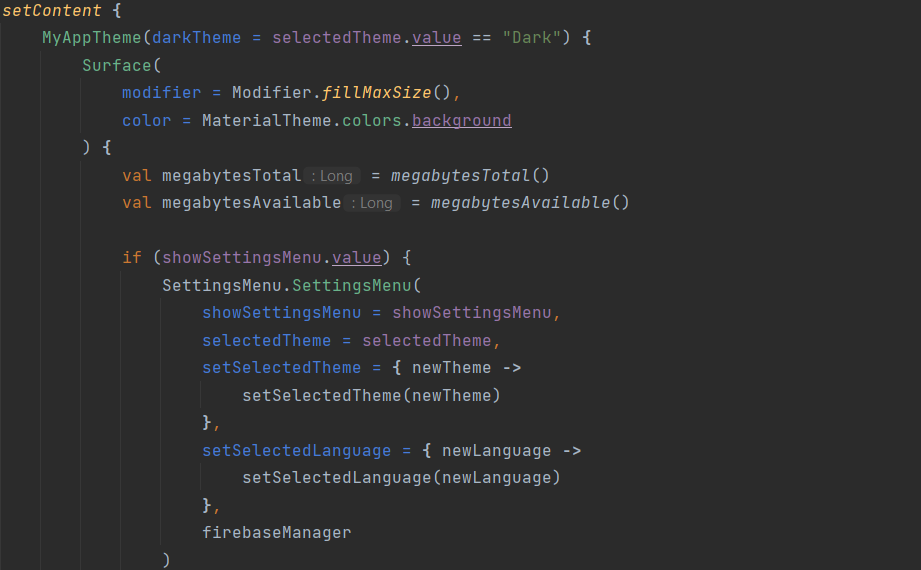
\includegraphics[height=240pt, width=260pt]{setContent1.png}
    \end{minipage}\hfill
    \begin{minipage}{0.45\textwidth}
        \centering
        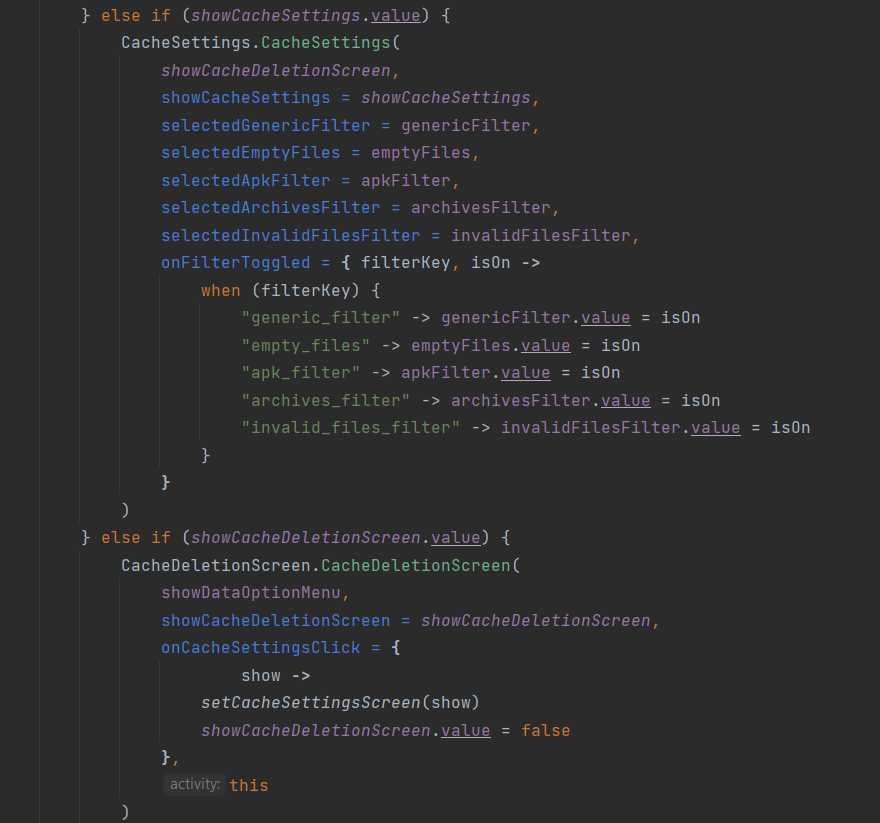
\includegraphics[width=260pt]{setContent2.png}
    \end{minipage}
    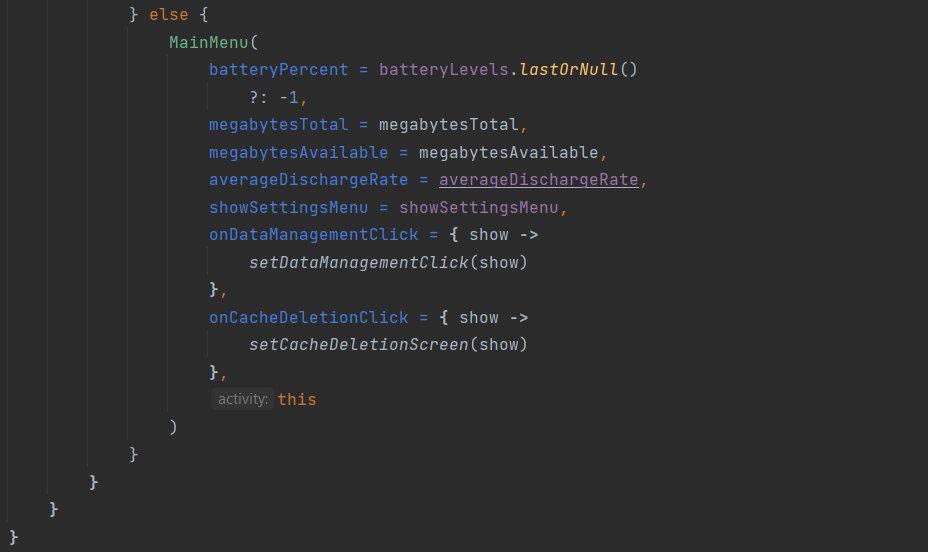
\includegraphics[width=260pt]{setContent3.png}
    \caption{Set Content}
    \label{fig: SetContent}
\end{figure}

Figure 4.1 shows the logic behind screen hopping, the app is actually composed of only two activities, the main activity and the permission activity, the content of the main activity being created through the setContent() method.

As such, the main activity sets up screens and values for whether these screens are shown or not. The main screen is the main menu, where the user accesses the other screens. Each screen is built with a composable, with the bulk of the \ac{UI} elements being comprised of Material3 elements.



\newpage
\begin{figure}[htp]
    \centering
    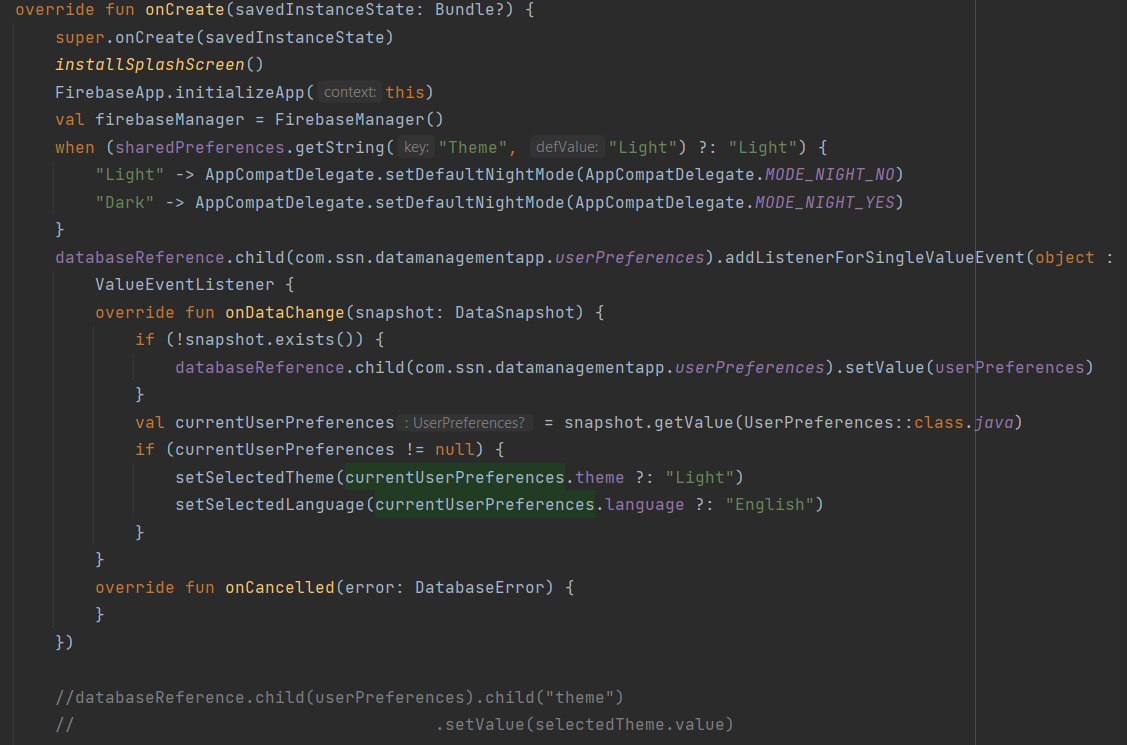
\includegraphics[width=380pt]{Firebase1.png}
    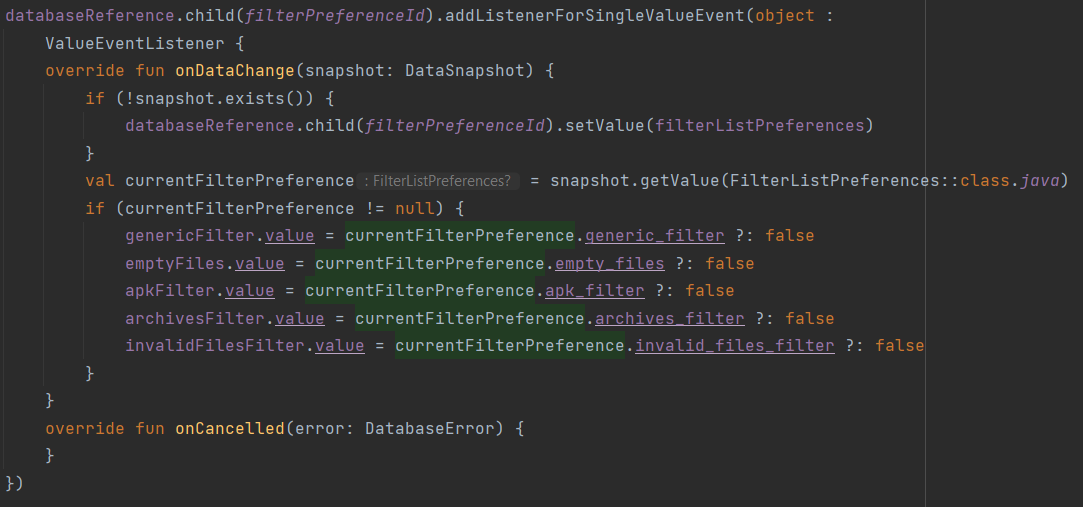
\includegraphics[width=380pt]{Firebase2.png}
    \caption{Firebase fetch \& update data}
    \label{fig: Firebase fetch & update data}
\end{figure}

In the above figure, 4.2, the onCreate function is called, which is a function usually called when first entering the application. It is here the basic logic of the application takes place, like the Firebase setup and preference assignation.

After which, we can see how the FirebaseApp is initialized, how the app selects the theme when the application is started, and how the data for the user preferences is being assigned at the beginning of the app, the values being assigned from the databaseReference value. At the beginning of the onDataChange method, if the collection userPreferences doesn't exist, if so, the app creates it. Then, the app assigns the current value for each preference value and updates the \ac{UI} accordingly.

Below it, the same operation is taking place for the preferences set by the user for the file filters that will be used for the cache deletion screen.
\newpage

\begin{figure}[htp]
    \centering
    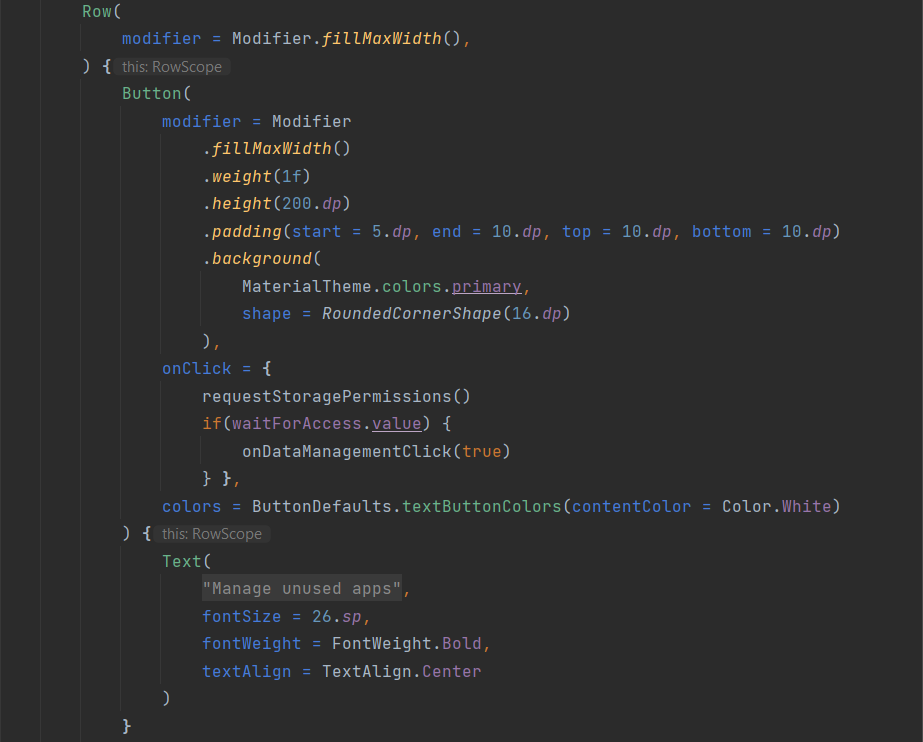
\includegraphics[width=460pt]{buttonexample.png}
    \caption{Button Implementation Example}
    \label{fig: Button Implementation Example}
\end{figure}

Here, figure 4.3, shows an example of the implementation of a button for menu hopping between the screens of the application. Most buttons throughout the app have a similar structure, utilizing Material3 elements, and the logic set up in the Main Activity for going through different menus.

For better alignment, a row composable is added, with a modifier to fill the maximum width of the screen. The button is then created, utilizing a button compose of the following variables: modifier, which is used for the shape of the button and the background color of it, onClick, which is used for managing the action that takes place when the button is clicked, and colors, which is used to color the text composable inside the button. The text composable has set up custom text alignment, custom font size, and weight, and for the text itself, the app uses the following method: context.getString(R.string.textdatamanagement), context is used as an instance for the current activity that is running, while R.string is used by the app to communicate with the file strings.xml, which holds various strings for ease of use and ease of potentially changing the application's language.

\newpage

\subsection{Settings Menu Implementation}\label{subsect:Settings Menu Implementation}

\begin{figure}[htp]
    \centering
    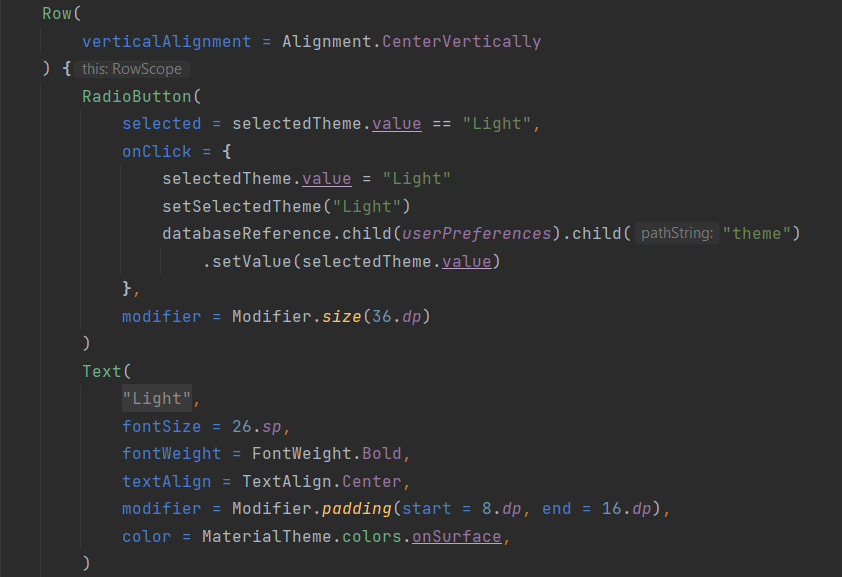
\includegraphics[width=380pt]{light.png}
    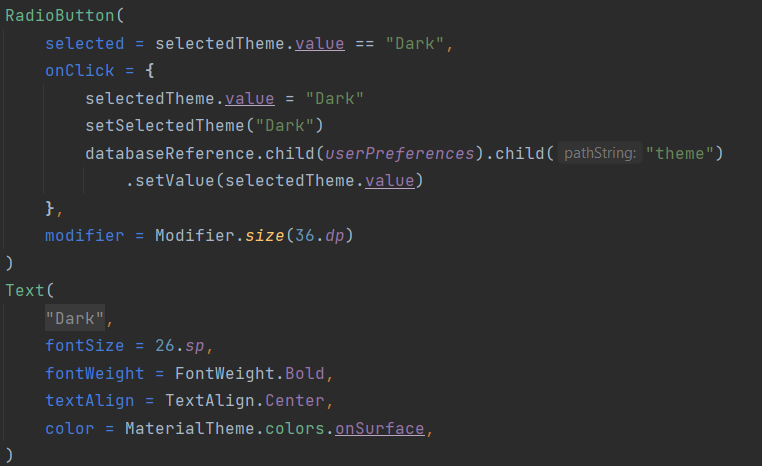
\includegraphics[width=380pt]{dark.png}
    \caption{Theme Options}
    \label{fig: Theme Options}
\end{figure}

Figure 4.4 showcases the implementation of theme options. For that, a set of radio buttons was preferred, the first radio button being used for the light theme, while the second being used for the dark theme. After clicking on one of the radio buttons, the other button is closed, and the changes are updated as well in the Firebase Database, where the theme value is updated accordingly.

SelectedTheme is used as a way to check which radio button should be checked, while setSelectedTheme is used to set for the whole app the new theme is chosen.

As mentioned in the explanation of Figure 4.3, the way these elements are created consists of composable functions, each having the benefit of being easy to use.

\newpage

\begin{figure}[htp]
    \centering
    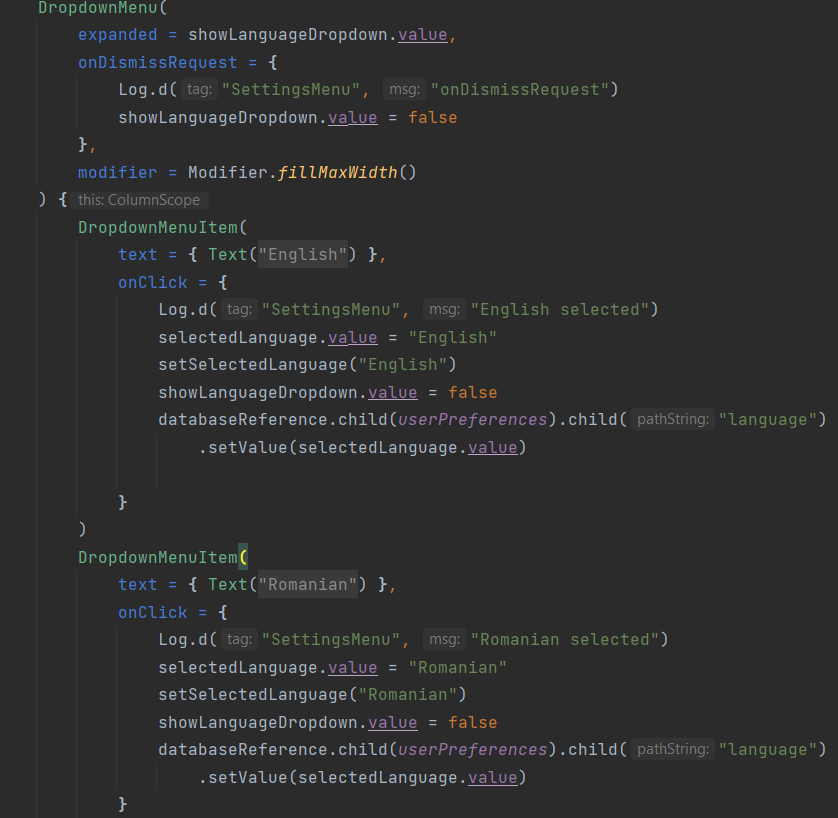
\includegraphics[width=450pt]{language.png}
    \caption{Language Dropdown Menu}
    \label{fig: Language Dropdown Menu}
\end{figure}

Here, in Figure 4.5 can be seen the implementation for the language dropdown menu, where the user can choose either Romanian or English as the preferred language for the application.

A DropdownMenu composable was used to achieve this, the menu showing up only when the user clicks on an icon with a text called Language, and closing after the user chooses a language. The menu is populated by items made with the composable DropdownMenuItem which hold text and a clickable button that selects the new language and calls a function inside the main activity that changes the text to the desired language.

\newpage

\begin{figure}[htp]
    \centering
    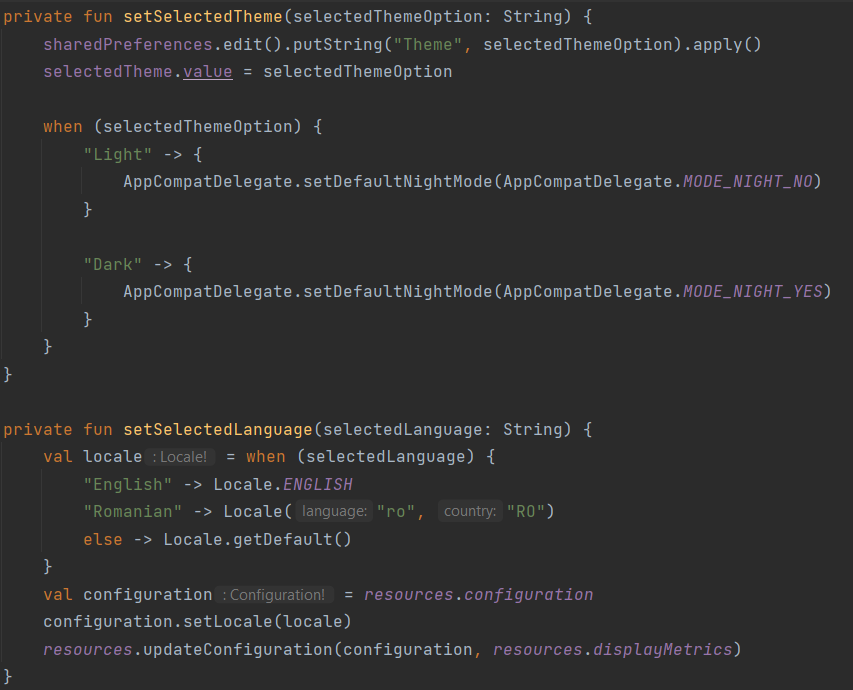
\includegraphics[width=460pt]{setPreferences.png}
    \caption{Theme Options}
    \label{fig: Applying the preferences}
\end{figure}

Figure 4.6 showcases how the language and theme are being applied, the code being found in the main activity class.

For the theme, the main activity looks at the sharedPreferences and edits them by applying the new selected theme. If the theme is selected as light, the app turns off night mode, while if the theme selected is the dark one, the night mode is turned on.

The language is applied by selecting the Locale as either English or Romanian, this object is used to define what language, symbols, and so on should be used.

\newpage

\subsection{Cache Deletion Screen Implementation}\label{subsect:Cache Deletion Screen Implementation}

\begin{figure}[htp]
    \centering
    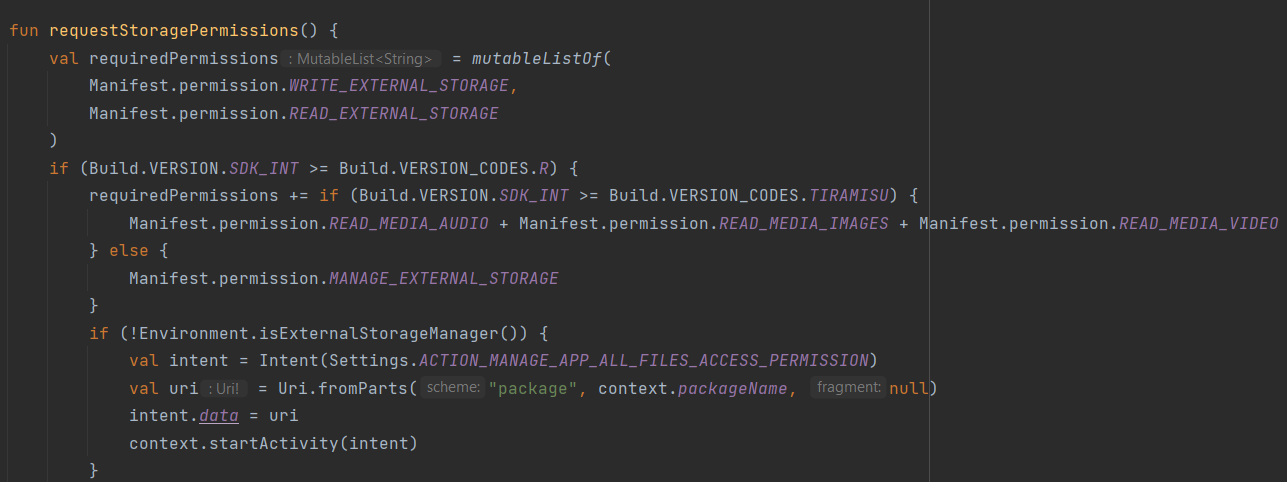
\includegraphics[width=400pt]{permission1.png}
    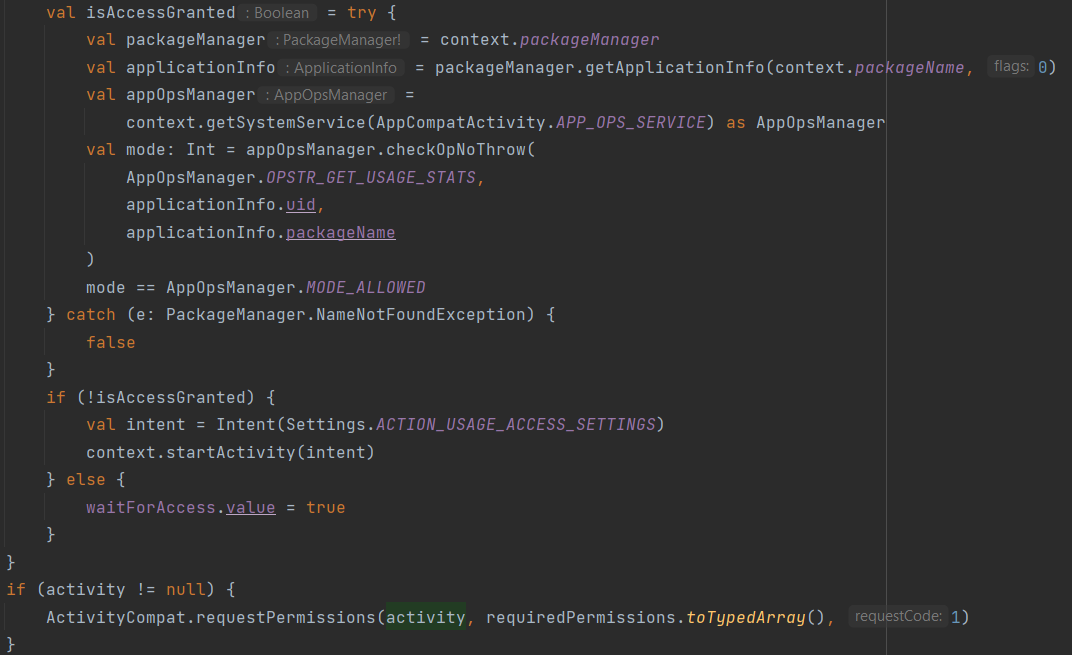
\includegraphics[width=400pt]{permission2.png}
    \caption{Permission Activity}
    \label{fig: Permission Activity}
\end{figure}

Firstly, the application requires some permissions from the user. As such, the above figure shows the logic for asking for such permissions. Firstly, it checks the Android version and adds the required permissions to a list. It then checks if the usage access is granted and starts an activity to request permission if it is not granted. Lastly, the function uses ActivityCompat.requestPermissions to request storage permissions from the user.

\newpage

\begin{figure}[htp]
    \centering
    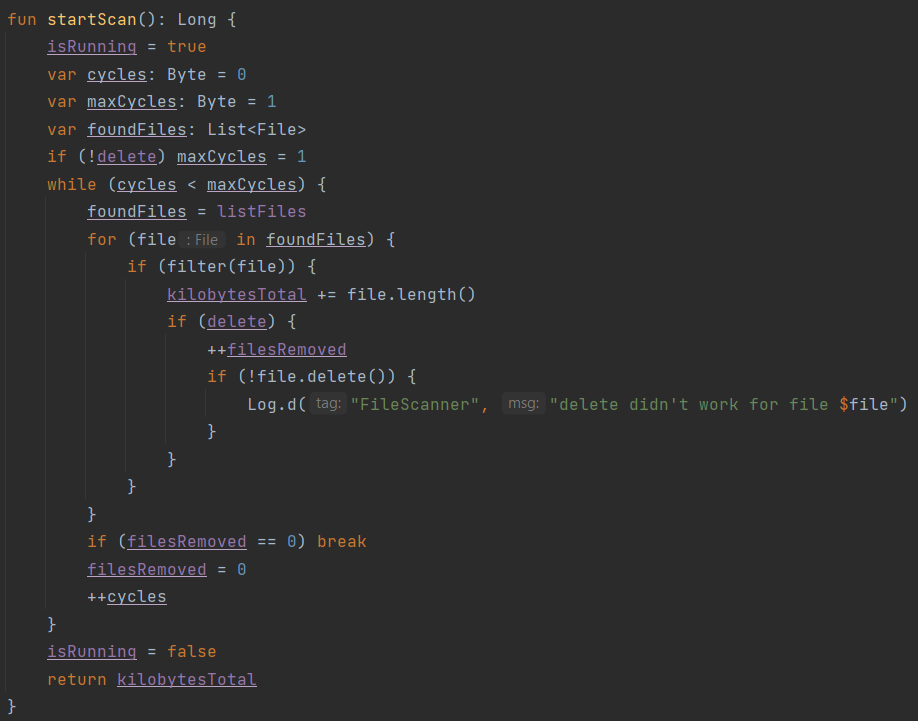
\includegraphics[width=290pt]{cache 1.png}
    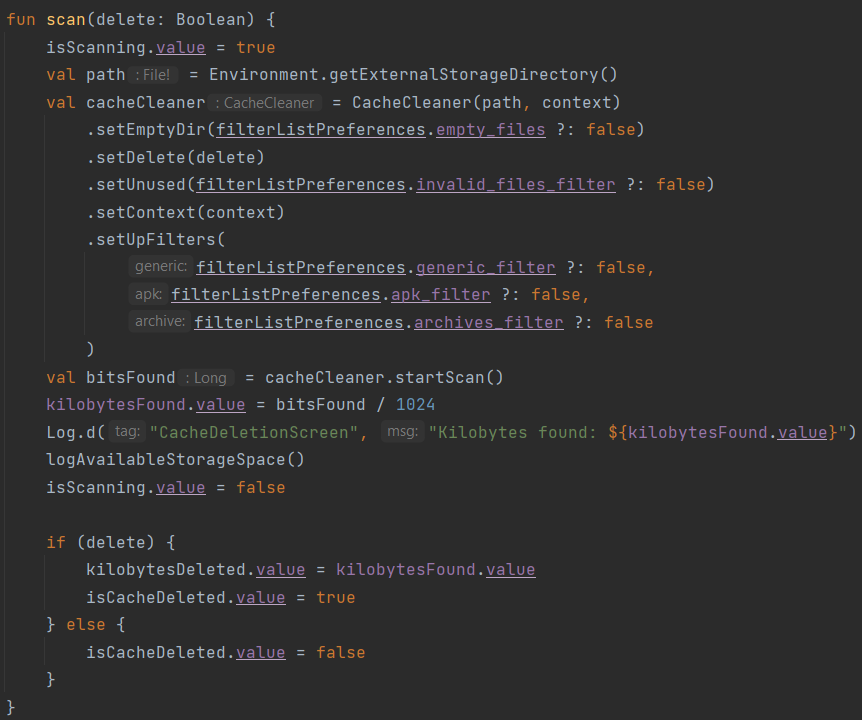
\includegraphics[width=290pt]{cache 2.png}
    \caption{File Scanner}
    \label{fig: File Scanner}
\end{figure}

The Cache Screen consists of two main buttons, analyze and delete. Both of these buttons are created using compose functions like text, buttons, and so on. However, the main point of this app is the scanning feature. As such, when the user presses one of the buttons, the app utilizes the function defined in Figure 4.8. 

Scan() gets the general path of the external storage and creates an instance of the CacheCleaner class that sets up various filters for the type of files the user wants to delete and passes a value for delete, whether the user wants to remove or not the files scanned. To compute the number of kilobytes found, the method uses the CacheCleaner instance to start another function for the proper scanning.

The function startScan() first creates a list of all the files in the storage and then begins going through each one and selecting only those that have their respective filter set on. If the delete value is set to true the removing process can begin and all selected files are deleted from the system. Finally, the app returns the amount of memory it has freed up.
\newpage

\subsection{Unused App Screen Implementation}\label{subsect:Unused App Screen Implementation}


\begin{figure}[htp]
    \centering
    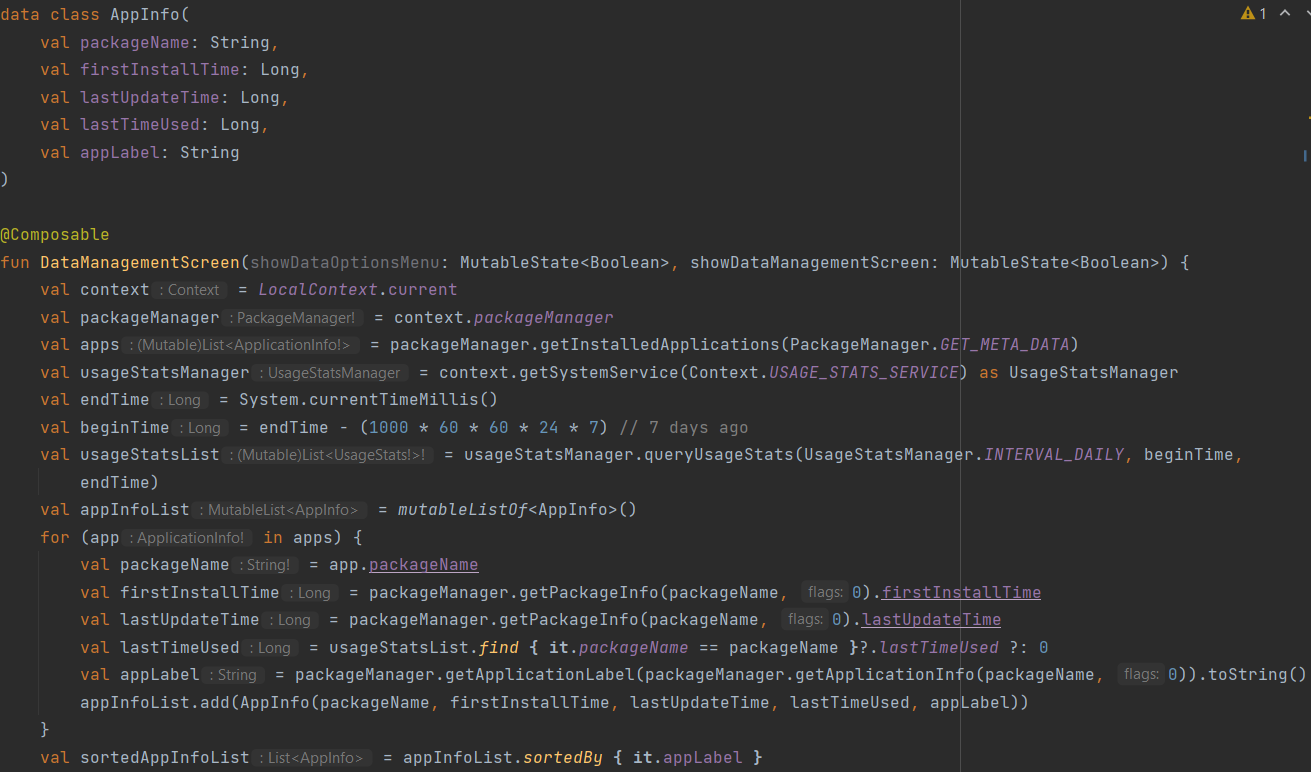
\includegraphics[width=340pt]{unused.png}
    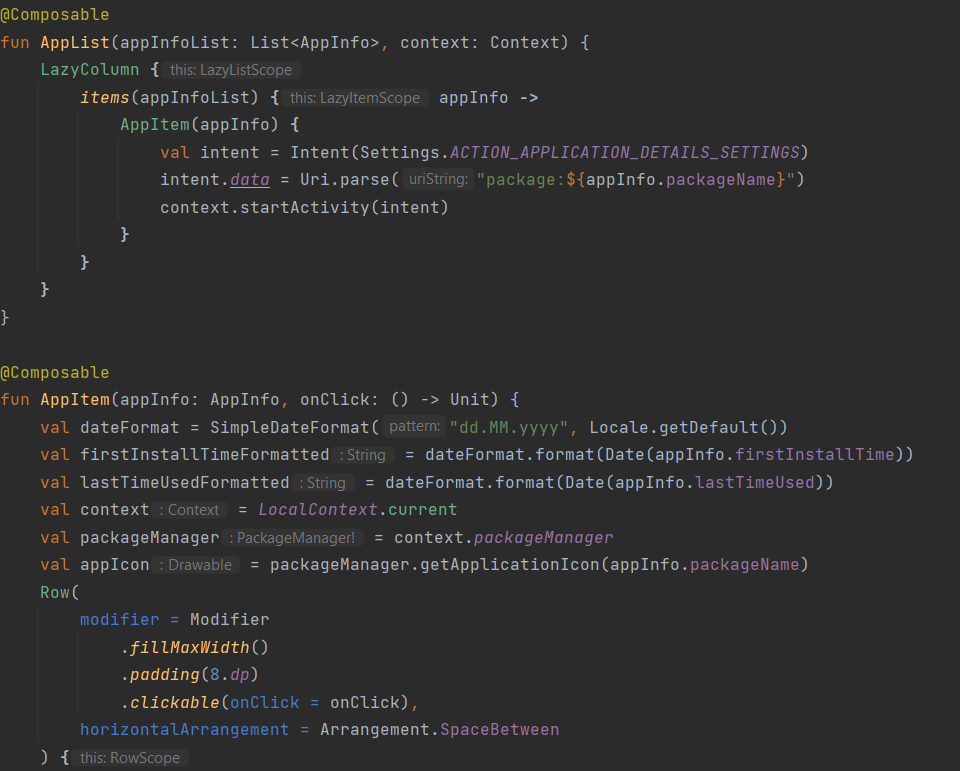
\includegraphics[width=340pt]{unused2.png}
    \caption{File Scanner}
    \label{fig: File Scanner}
\end{figure}

The following Figure, 4.9, shows the logic behind the unused app list. The app list is given through a package manager which retrieves all applications which are then sorted by alphabetical order. The usage stats manager retrieves all the information on when the application was used, when was it installed and when was it last updated.

The composable function AppList assigns to each app their respective app info screen so that when one of the applications in the list is clicked, the app info activity and screen are opened.

AppItem is used to create the visual representation for each application in the list.

\newpage

\subsection{Trash Emptying Implementation}\label{subsect:Trash Emptying Implementation}

\begin{figure}[htp]
    \centering
    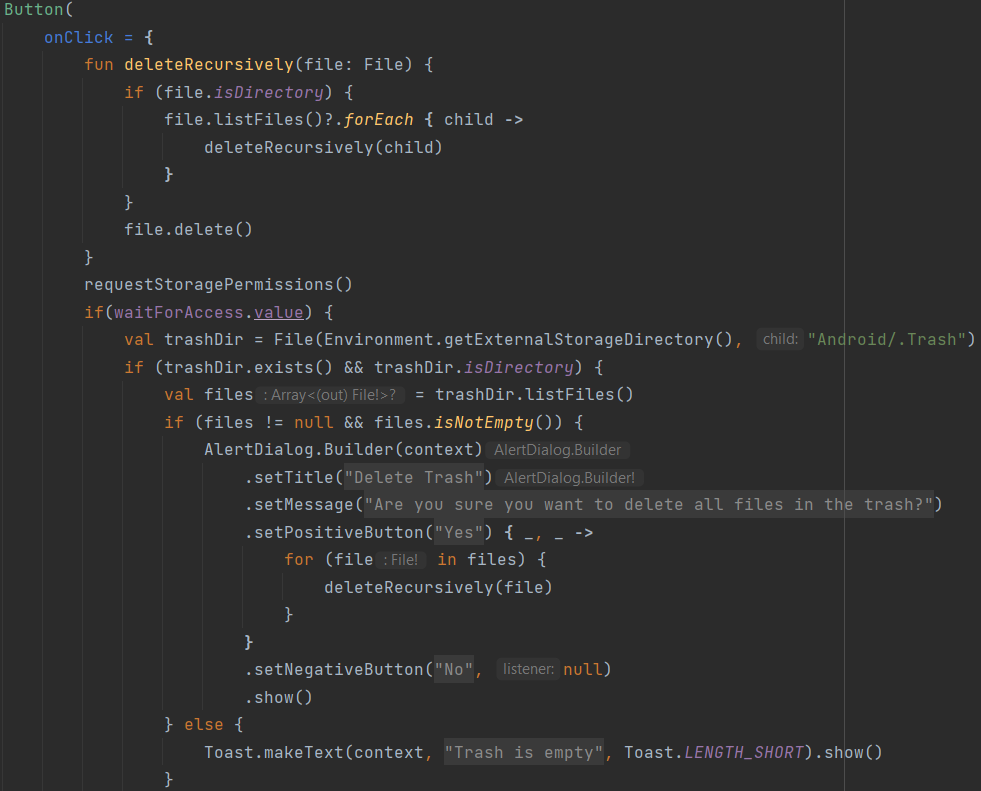
\includegraphics[width=450pt]{trash1.png}
    \caption{App Info}
    \label{fig: Emptying trash logic}
\end{figure}

The last Figure, 4.10, shows the logic for emptying the trash folder, it first requires the needed permissions, and if they are granted, the app will check for the existence of the trash directory. If it exists, the app lists the files inside it and starts recursively deleting them after creating an alert menu. If no apps are found, the application creates a toast composable, a pop-up message, saying that the trash is empty.


\newpage
